% To add:
% 1. Density section, fits, values, widths, etc.
% 2. interfacial width by shear rate plot for tetrahedrality
% 3. interfacial width by shear rate plot for density?

\chapter{STRUCTURAL WIDTHS OF ICE-I$_\mathrm{h}$ / WATER INTERFACES}\label{chap:Str}
One of the open questions about ice / water interfaces is whether the
thickness of the interfacial `slush' layer depends on the facet of ice
presented to the water. In the interfacial region, the water molecules
are ordered differently than in either the solid or liquid phases, and
also exhibit dynamics unique to their local structure.  The width of
this interfacial layer has been estimated by finding the distance over
which structural order parameters or dynamic properties change from
their bulk liquid values to those of the solid ice. The properties
used to find interfacial widths have included the local density, the
diffusion constant, and both translational and orientational order
parameters~\cite{Karim1988,Karim1990,Hayward2001,Hayward2002,Bryk2002,Gay2002,Louden2013a}.The
VSS-RNEMD method employed here creates thermal and velocity gradients
in the system, during which the momenta of the water molecules are
perturbed, thus any order parameters that depends on translational
motion may measure the momentum exchange and not physical properties
of the interface. To avoid these influences, we have probed the
ice-I$\mathrm{h}$ / water interface by observing the transition of
several order parameters from their ice to bulk liquid values.  In
this chapter, we focus on structural measures of the ice / water
interface. Dynamic measures are investigated later in Chapter
\ref{chap:Dyn}.

\section{Density Measurements Transverse to the Interface}
Following the pioneering work of Haymet \textit{et al.}, we initially
probed the ice-I$_\mathrm{h}$ / water interface by examining the
transition of the density of molecules from bulk liquid to bulk
ice. Four consecutive 1 ns simulations of quiescent ice / water
systems were performed for each interface. The simulations were
performed under a constant volume and constant energy integrator
(NVE), equilibrated at the coexistence temperature (225~K for SPC/E
and 270~K for TIP4P/Ice) and with no VSS-RNEMD moves attempted
(\textit{i.e.} no thermal or momentum flux applied). During the
simulations, the positions and velocities of the water molecules were
sampled every 0.1 ps.

To compute transverse density profile, each frame of the trajectories
were divided into 0.25~\AA bins, and the average density of each bin
was accumulated. The density profiles were then fit with a hyperbolic
tangent function designed to smoothly transition between the bulk
liquid and ice domains. Following Haymet \textit{et al.}, only the
density maximas corresponding to the planes of ice were included in
the data to be fit.
\begin{equation}\label{rho_fit}
\rho (z) \approx
\rho_\mathrm{liq}+\frac{\rho_\mathrm{ice}-\rho_\mathrm{liq}}{2}\left[\tanh\left(\frac{z-l}{w^\rho}\right)-\tanh\left(\frac{z-r}{w^\rho}\right)\right]
\end{equation}
Here, $\rho_\mathrm{liq}$ and $\rho_\mathrm{ice}$ are the densities of
the liquid and ice respectively. The $z$-locations of the left and
right Gibbs dividing surfaces are $l$ and $r$, and $w^\rho$ is the
width of the interface. An example density profile for each of the
SPC/E interfaces is shown in Figure \ref{fig:transDensity} (a similar
graph for the TIP4P-Ice results can be seen in Figure
\ref{fig:TIPtransDensity} in Appendix \ref{structAppendix}).

\begin{figure}[H]
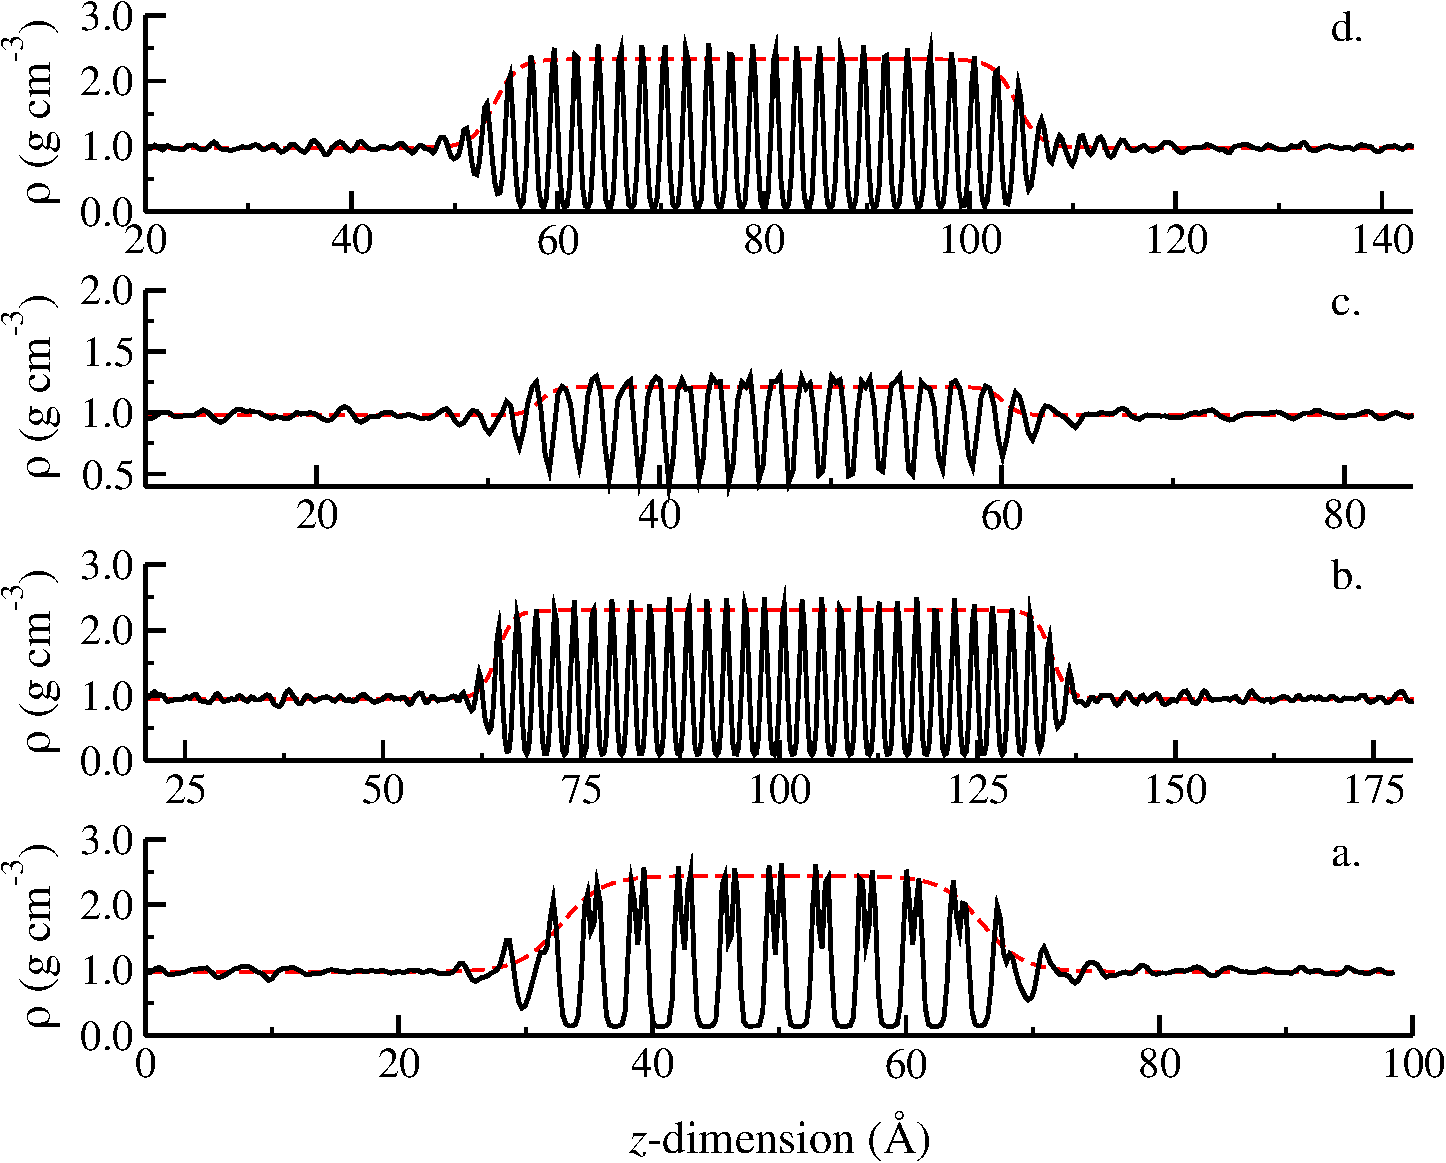
\includegraphics[width=\linewidth]{Figures/transDensity}
\caption{\label{fig:transDensity}Transverse density profiles for the
  basal (a), prismatic (b), 14\degree~pyramidal (c) and secondary prism (d)
  facets of an SPC/E ice-I$_\mathrm{h}$ / water interface (black
  lines). The prismatic and secondary prism profiles are zoomed in to
  show detail at the ice / water interface. The profiles are fit using
  Eq. \eqref{rho_fit} (dashed red lines).}
\end{figure}

From Eq. \eqref{rho_fit}, we have obtained estimates for $w^{\rho}$;
these values are related to the $10\%-90\%$ interfacial widths
commonly reported in previous studies
($w_\mathrm{10-90}^{\rho} = 2.197~w^{\rho}$).\cite{Bryk2002,Bryk2004}
For the SPC/E interfaces at 225~K, we find large discrepencies in
$w_\mathrm{10-90}^{\rho}$ as seen in Table \ref{tab:strWidths}.

\begin{table}[h]
\centering
\caption{COMPUTED WIDTHS OF THE ICE-I$_\mathrm{h}$ / WATER INTERFACES BY
  STRUCTURAL MEASURES. \label{tab:strWidths}} 
\begin{tabular}{|r|cc|cc|}  
\hline
  \multirow{2}{*} & \multicolumn{2}{c|}{SPC/E (225~K)} &  \multicolumn{2}{c|}{TIP4P/Ice (270~K) } \\
  & \multicolumn{2}{c|} {Interfacial Widths (\AA) \footnotemark[1]} &
                                                                      \multicolumn{2}{c|} {Interfacial Widths  (\AA) \footnotemark[1]} \\
 Interface &  $w_\mathrm{10-90}^{\rho}$ & $w_\mathrm{10-90}^{q}$ &  $w_\mathrm{10-90}^{\rho}$ &  $w_\mathrm{10-90}^{q}$ \\ 
\hline
  Basal  $\{0001\}$                 & 9(1) & 7.5(4) & 8.1 & 8.8(8)  \\
  Prismatic  $\{10\bar{1}0\}$       & 7(2)  & 7.2(2) & 9.2 & 9.0(5)  \\
  14\degree~Pyramidal  $\{20\bar{2}1\}$       & 3.1(6) & 6.6(2) & 4.6 & 8.2(5)  \\
  Secondary Prism  $\{11\bar{2}0\}$ & 8(1) &6.7(2) & 8.0 & 9.4(6)  \\ 
\hline
\end{tabular}
\flushleft
  \footnotemark[1]\footnotesize{Uncertainties in the last
   digit are indicated with parentheses.} \\
\end{table}

For the basal interface, $w_\mathrm{10-90}^{\rho} \sim$ 7 \AA~, where
values closer to 5 \AA~ are observed for the prismatic and secondary
prism interfaces. Lastly, the density transition occurs over $\sim$ 2
\AA~ for the 14\degree~pyramidal interface. Since the
14\degree~pyramidal crystal does not have well defined
crystallographic planes perpendicular to the dimension normal to the
surface, fitting the resulting density profiles gives skewed
results. Values for $w_\mathrm{10-90}^{\rho}$ for the TIP4P/Ice
systems are also reported in the same table. While the interfacial
width is observed to be larger for the TIP4P/Ice model, this is
primarily due to the warmer coexistence temperature. It is evident
from the density profiles and fits in Figure \ref{fig:transDensity}
that an order parameter that does not depend on the crystal
orientation would give a more accurate estimate of the ice / water
interface. 

\section{Local Tetrahedral Order Parameter}
As a second structural measure of the interface, we have used the
local tetrahedral order parameter, which compares the local molecular
environments (e.g. the angles between nearest neighbor molecules) to
perfect tetrahedral ordering. This method would not be skewed due to
rotations of the crystal, and would therefore more accurately quantify
the transition of the local structure through the interface. This
quantity was originally described by Chau and
Hardwick,~\cite{Chau1998} was rescaled by Errington and
Debenedetti,~\cite{Errington2001} and has been used in bulk liquid
simulations by Kumar \textit{et al.}~\cite{Kumar2009} It has also
previously been used in ice / water interfaces by Bryk and
Haymet~\cite{Bryk2004}, and in our initial work on ice / water
interfaces\cite{Louden2013a}.

We have evaluated the local tetrahedral order parameter, $q$, along
the coordinate perpendicular to the ice / water interface, i.e., the
$z$-axis of the simulation box. With $N$ molecules,
\begin{equation}
q(z) = \frac{1}{N_z} \int_0^L \sum_{i=1}^{N} \Bigg(1 -\frac{9}{2n(n-1)}\sum_{j=1}^{n-1}
\sum_{k=j+1}^{n} \bigg(\cos\psi_{jik}+\frac{1}{3}\bigg)^2\Bigg)
\delta(z_{i}-z)\mathrm{d}z .
\label{eq:qz}
\end{equation}
$\psi_{jik}$ is the angle formed between the oxygen sites of water
molecules $i$, $j$, and $k$, where molecule $i$ is the central water
molecule (with $n$ neighbors) and molecules $j$ and $k$ are two of the
neighbors of $i$.  The neighboring molecules $j$ and $k$ are
restricted to lie within the first solvation shell of molecule $i$
($r < 3.41$~\AA\ for water), and the double sum visits all angles for
the $n$ neighbors of molecule $i$ that are within this distance.  When
molecule $i$ has exactly four neighbors ($n=4$), the prefactor reduces
to $3/8$, as in the expression of Errington and Debenedetti, but
Eq. \eqref{eq:qz} also provides tetrahedrality information for water
molecules that are either under- or over-coordinated. We have also
introduced the normalization factor
$N_z = \sum_i \int \delta(z_i - z) \mathrm{d}z$ to account for the
varying populations of water molecules within each finite-width bin.

At low temperatures, the tetrahedral order parameter can approach
unity for perfect ice-I$_\mathrm{h}$ structures. However, at
temperatures close to melting, values of 0.9 are more common in SPC/E
ice due to thermal motion in the lattice. In the liquid, overlap of
the local environment with a perfect tetrahedron is reduced, and
values of $q(z) \approx 0.75$ are common in SPC/E water at 225~K. The
results indicate more tetrahedral structure in TIP4P/Ice; at
270~K, tetrahedrality averages, $q(z) \approx 0.95$ and $0.75$ are
found in the ice and liquid, respectively.

The structural widths of the ice / water interfaces were determined by
dividing each system into 1~\AA~ bins along the $z$-axis, and
computing statistical averages of $q(z)$ in each bin. For the
secondary prism interface (using SPC/E water at 225~K), the resulting
distribution can be seen in the bottom panel of Fig. \ref{fig:spComic}
(and in the Supporting Information for the other interfaces and
TIP4P/Ice). In the bulk liquid (at small and large values of $z$), the
order parameter takes on values of $q(z) \approx~0.77$, while
$q(z) \approx~0.92$ was found in bins spanning the ice. The
tetrahedrality profiles were fit using the same function as the
density profiles, however, an additive term was include to account for
the change in tetrahedral ordering due to the thermal gradient
throughout the system (turquoise line in the
bottom panel of the same figures),
\begin{equation}\label{tet_fit}
q(z) \approx
q_\mathrm{liq}+\frac{q_\mathrm{ice}-q_\mathrm{liq}}{2}\left[\tanh\left(\frac{z-l}{w^q}\right)-\tanh\left(\frac{z-r}{w^q}\right)\right]+\beta\left|z-\frac{r+l}{2}\right|.
\end{equation}
Here $q_\mathrm{liq}$ and $q_\mathrm{ice}$ are the values of the order
parameter for the bulk liquid and ice domains. The locations $l$ and
$r$ are the $z-$coordinates of the Gibbs dividing surface for the left
and right interfaces (shown in Fig. \ref{fig:spComic} with vertical
dotted lines), and $w^{q}$ is the interfacial width.  The last term in
Eq. \eqref{tet_fit} accounts for the influence of the weak thermal
gradient on the tetrahedrality profile in the liquid region. Namely,
at warmer temperatures the liquid is able to adopt local
configurations resulting in lower values of the order parameter. This
results in a small linear decay in the tetrahedrality profiles for
increasing displacements from the ice surface.

\begin{figure}
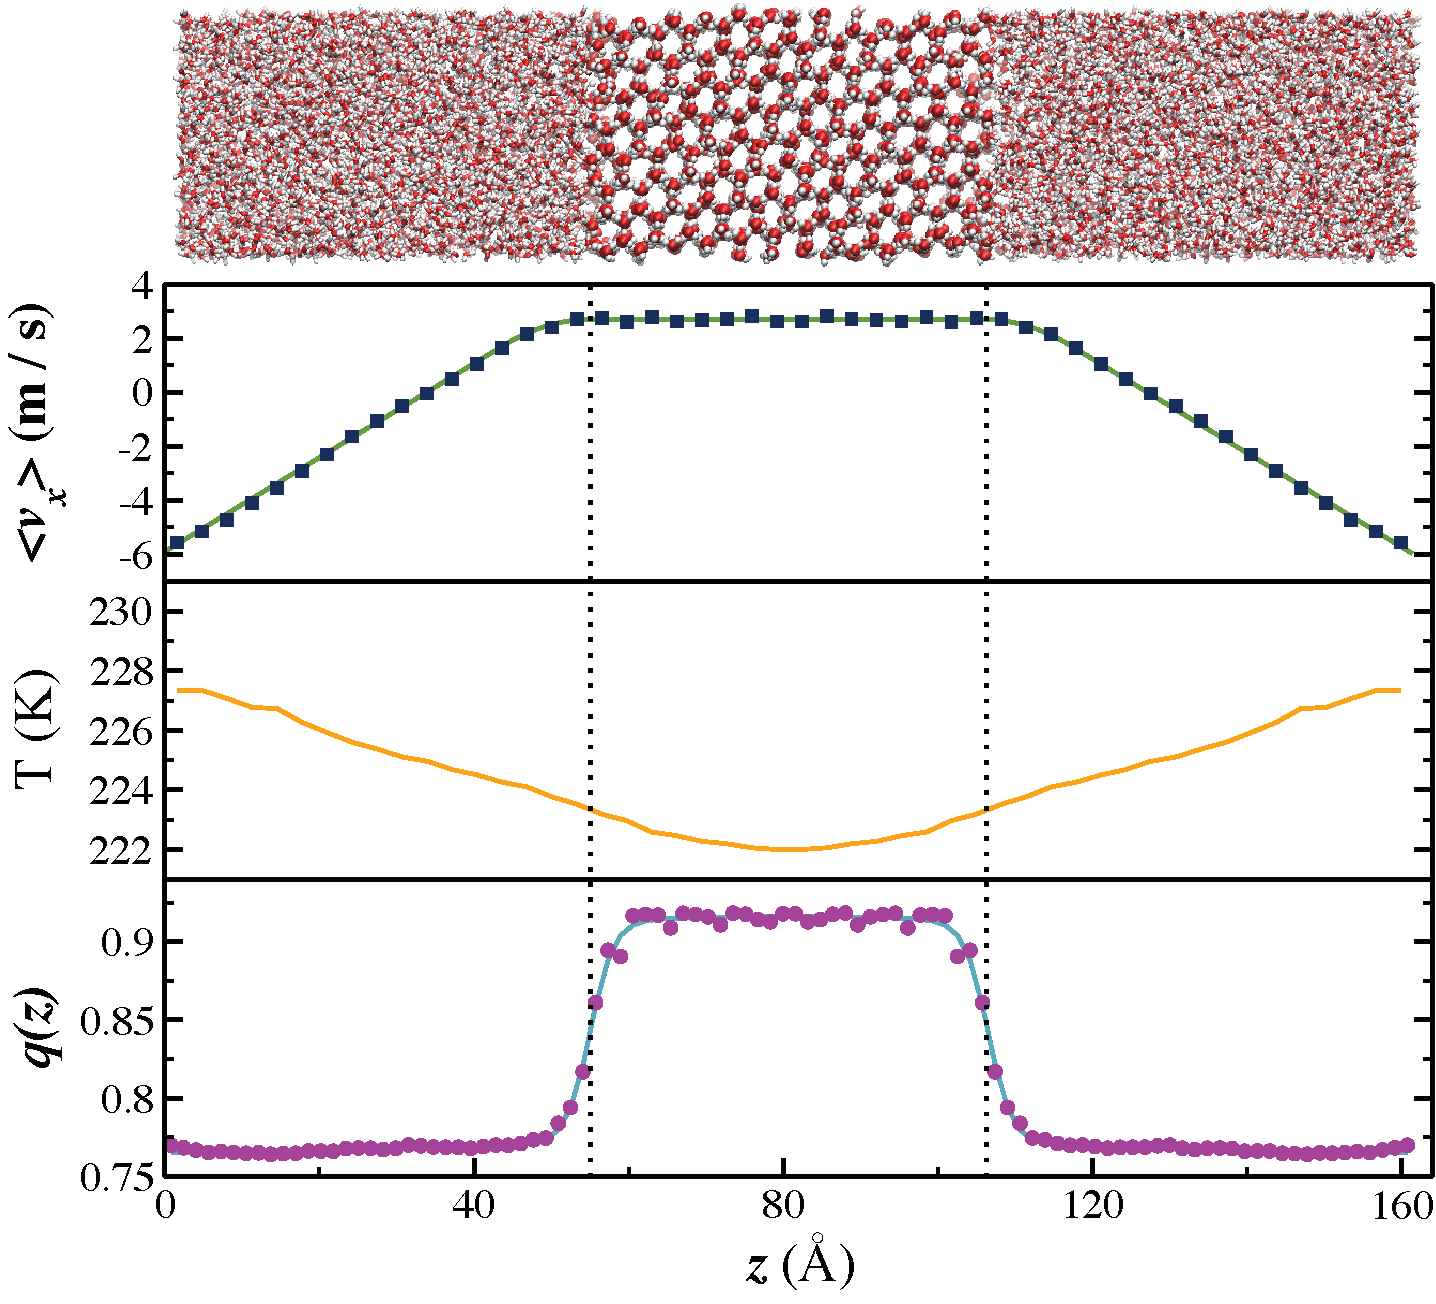
\includegraphics[width=\linewidth]{Figures/SecPrismComicStrip}
\caption{\label{fig:spComic} Properties of the secondary prism
  interface (top) being sheared through water at 8.6 m
  s\textsuperscript{-1}. Lower panel: the local tetrahedral order
  parameter, $q(z)$, (circles) and the hyperbolic tangent fit
  (turquoise line).  Middle panel: the imposed thermal gradient
  required to maintain a fixed interfacial temperature of $\sim$225 K
  with the SPC/E water model. Upper panel: the transverse velocity
  gradient (squares) that develops in response to an imposed momentum
  flux, along with the fit (green line). The vertical dotted lines
  indicate the locations of the Gibbs dividing surfaces of the two
  interfaces.}
\end{figure}

In the middle panel of Fig. \ref{fig:spComic}, we show the resulting
thermal gradient from the imposed kinetic energy flux. For the SPC/E
water model, the interfacial temperature is held at $\sim$ 225~K
(270~K for the TIP4P/Ice), allowing investigation of the response to
the shear while maintaining solid / liquid coexistence. In the top
panel, the velocity gradient resulting from the imposed momentum flux
shows that the ice has a uniform positive velocity along the $x$
axis. The bulk liquid at the ends of the simulation cell has negative
velocity, although the center of mass of the simulation box is
stationary.  The bulk fluid shows a primarily linear velocity gradient
allowing for easy calculation of the shear viscosity using
Eq. \eqref{eq:viscosity}. Close to the interface, the ice imparts
significant positive momentum into the surrounding interfacial liquid.
Projections of the velocity gradient from the liquid onto the Gibbs
dividing surface indicate that the ice-water interface is in the
negative slip regime. For comparison, Figure \ref{fig:tipsComic} shows
the secondary prism interface for the TIP4P/Ice system.

\begin{figure}[H]
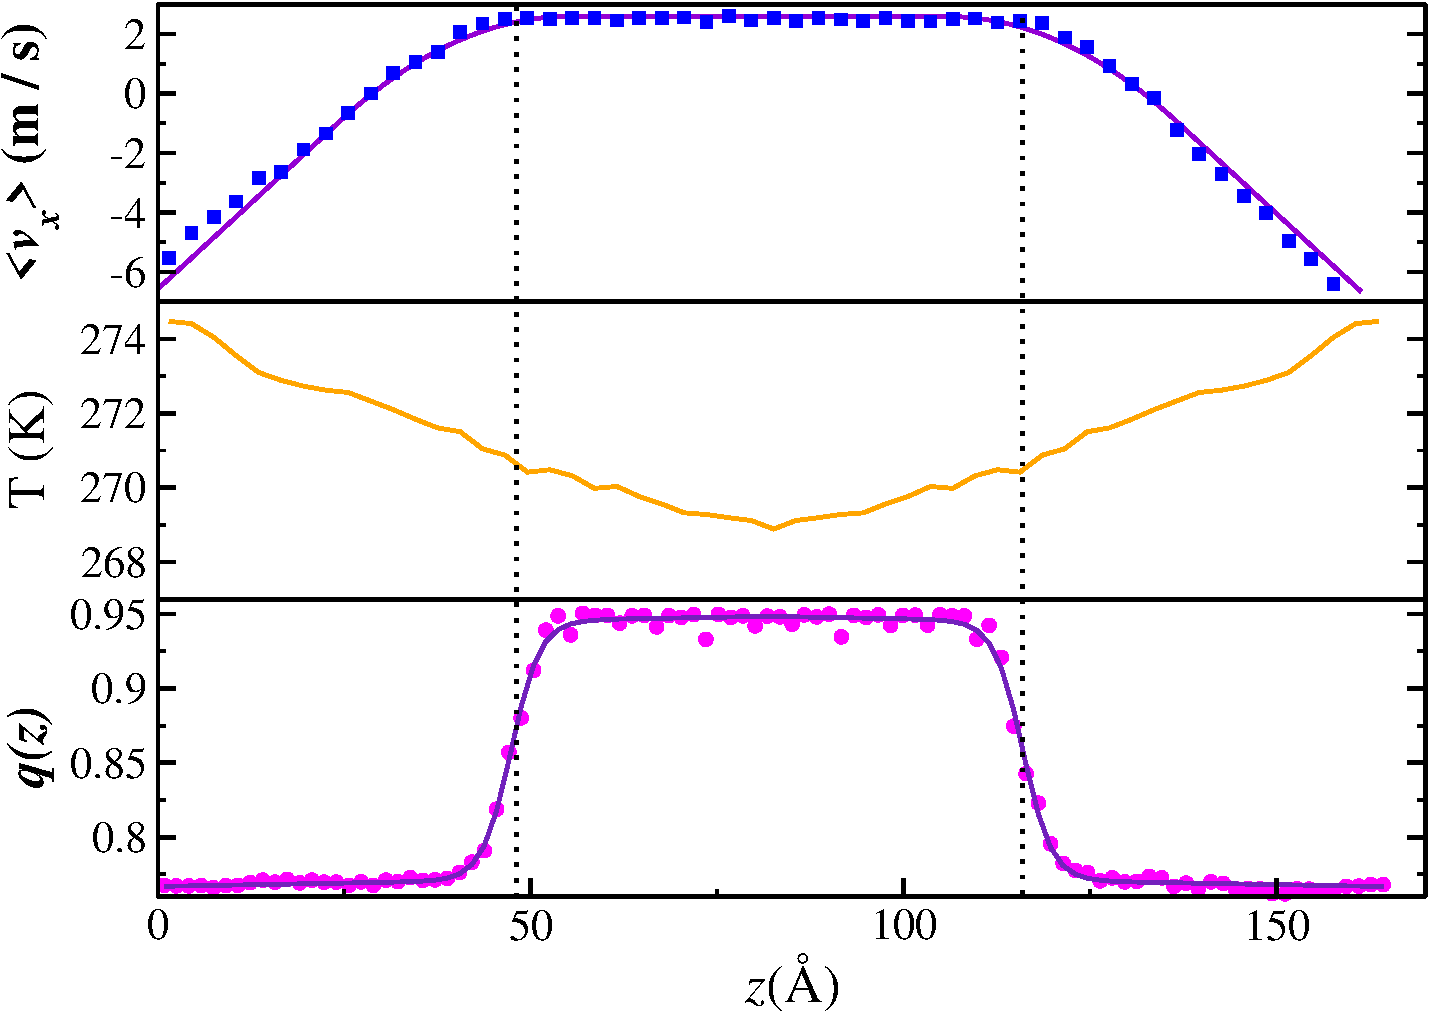
\includegraphics[width=\linewidth]{Figures/SecPrism_TIP4PIce_Plot}
\caption{\label{fig:tipsComic} Properties of the TIP4P/Ice secondary prism
  interface being sheared through water at 8.4
  ms\textsuperscript{-1}. Lower panel: the local tetrahedral order
  parameter, $q(z)$, (circles) and the hyperbolic tangent fit
  (blue line).  Middle panel: the imposed thermal gradient
  required to maintain a fixed interfacial temperature of 270 K. Upper
  panel: the transverse velocity gradient (squares) that develops in
  response to an imposed momentum flux, along with the fit (purple
  line). The vertical dotted lines indicate the locations of the Gibbs
  dividing surfaces of the two interfaces.}
\end{figure}

From Eq. \eqref{tet_fit}, we have obtained estimates for $w^{q}$, the
structural widths of the interfaces for the quiescent ice / water
systems. These values are related to the $10\%-90\%$ interfacial
widths commonly reported in previous studies
($w_\mathrm{10-90}^{q} = 2.197~w^{q}$).\cite{Bryk2002,Bryk2004} For the
SPC/E interfaces at 225~K, we find
$w_\mathrm{10-90}^{q} \approx 7$~\AA~ as seen in Table
\ref{tab:strWidths}. These values are similar to our previous findings
for the $10\%-90\%$ interfacial widths obtained from shorter
simulations, ($7.0 \pm 0.9$ \AA) for basal and ($7.9 \pm 0.4$ \AA) for
prismatic interfaces.\cite{Louden2013a} The interfacial widths in
TIP4P/Ice systems indicate slightly broader interfaces, where values
of $w_\mathrm{10-90}^{q} \approx 9$~\AA~ are more common. These values
are also reported in Table \ref{tab:strWidths}.

Over the range of shear rates investigated,
$\sim 0.5-10.0~\mathrm{~m~s}^{-1}$, we find no significant changes in
the interfacial widths for any of the crystal faces (see Fig. \ref{fig:tetByShearRate}). All values of
$w_\mathrm{10-90}^{q}$ obtained from shearing simulations fell inside the
error bars of the values obtained from the quiescent simulations.

\begin{figure}[H]
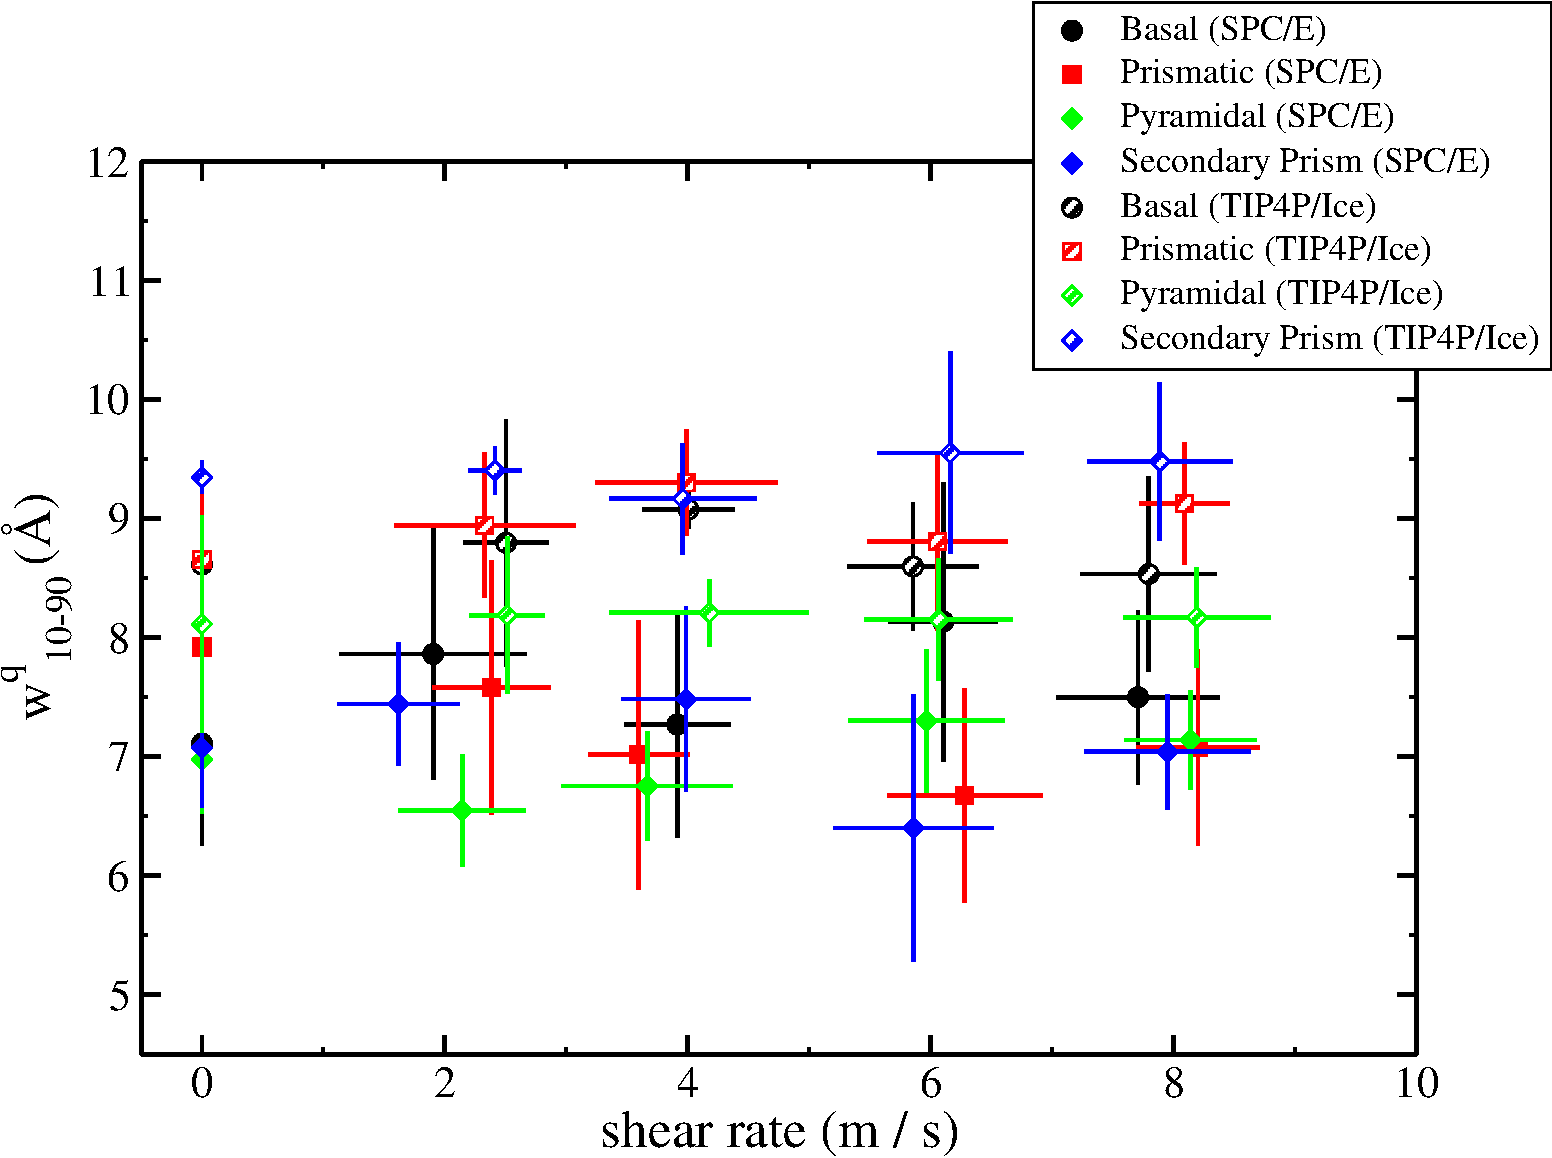
\includegraphics[width=\linewidth]{Figures/tetByShearRate}
\caption{\label{fig:tetByShearRate}The 10-90 widths of the
  ice-I$_\mathrm{h}$ / water interface for the basal, prismatic,
  14\degree~pyramidal, and secondary prism crystal faces as determined
  by the local tetrahedral order parameter fit by
  Eq. \eqref{tet_fit}.}
\end{figure}


\section{Discussion}
In their initial studies in the late 1980's, Karim and Haymet
investigated the liquid to solid transition for a basal
ice-I$_\mathrm{h}$ / water interface using the TIP4P model at
240~K.\cite{Karim1987,Karim1988} They divided their system into 0.2
\AA~ bins along the dimension normal to the interface, and computed
the average density for each of these bins. These density profiles
were segmented into 3.7 \AA~bins, which coincide with the spacing of
the crystallographic planes inside their ice crystal. Karim and Haymet
then estimated the width of the basal ice-I$_\mathrm{h}$ / water
interface to be $\sim$ 10 - 15 \AA~ by counting the number of these
wider bins. This result proved to be invarient of the exposed surface
area of the basal plane, as a simulation of equal length in time with
a factor of four larger presented surface area yielded the same
results.

In a follow up study, Karim, Kay, and Haymet investigated the same
interface using the SPC water model.\cite{Karim1990} The interface was
observed the be stable at 200~K over 300 ps under a microcanonical
integrator. The basal ice-I$_\mathrm{h}$ / water interface was
estimated to be of approximately the same width as determined
previously with the TIP4P water model, by the methods described
above. 

About 10 year later, the problem was revisited by Hayward and Haymet,
where a comparitive study of the basal, prism, 14\degree~pyramidal,
and $\{2\bar{1}\bar{1}0\}$ secondary prism ice-I$_\mathrm{h}$ / water
interfaces was conducted.\cite{Hayward2001} This was the
first computer investigation of the 14\degree~pyramidal, and
$\{2\bar{1}\bar{1}0\}$ secondary prism ice-I$_\mathrm{h}$ / water
interfaces, providing the initial insights to the structure and
dynamics of these higher-order crystal facet interfaces. These two
interfaces were found to be of particular interest as Type 1
antifreeze proteins in both winter flounder and shorthorn Sculpin
inhibit ice growth at these ice
surfaces.\cite{Knight2001,Wierzbicki1996,Haymet1998,Harding1999}

They observed a stable ice / water interface at 270~K over 300 ps
using the CF1 central force model. From these trajectories, they
estimated the 10-90 width of the ice / water interfaces measuring the
transition of two structural criteria, the translational order and a
Gaussian filtered translational order (average density). For each order
parameter studied, the systems were divided into $\sim$3 \AA~ bins
along the dimension normal to the interface (chosen here to be along
the $z$-axis), and the average of the parameter was computed for each
bin. A Gaussian filter was then applied to the Fourier transofrm of
the resulting order parameter profile. For example, for the
translational order profile $\rho (z)$,
\begin{equation}
g(k) = \int_{-n}^{n} \mathrm{exp}(-2\pi ikz)\rho (z)dz
\end{equation}
where $n$ is half of the box length in the direction normal to the
interface. The oscillations in $g(k)$ are then dampened with the
Gaussian filter,
\begin{equation}
g'(k) = g(k)\mathrm{wt}(k)
\end{equation}
where 
\begin{equation}
\mathrm{wt}(k)=\frac{1}{\sigma_{k}\sqrt{2\pi }}~\mathrm{exp}\Bigg(-\frac{1}{2\sigma_{k}^{2}}k^{2}\Bigg).
\end{equation}
Here, $2\sigma_{k}$ defines the resolution of the Gaussian. Inverse
Fourier transform of $g'(k)$ gives the filtered translational order
profile, $\rho '(z)$
\begin{equation}
\rho '(z) = \int_{-n}^{n} \mathrm{exp}(2\pi ikz)g'(k)dk
\end{equation}
which can be written as a convolution integral
\begin{equation}
\rho '(z) = \int_{-n}^{n} \mathrm{wt}'(z-z')\rho (z')dz'
\end{equation}
where
\begin{equation}
\mathrm{wt}'(z-z') = \frac{1}{\sigma
  \sqrt{2\pi}}~\mathrm{exp}\Bigg(-\frac{1}{2\sigma^{2}}(z-z')^{2}\Bigg)
\end{equation}
and the value of $\sigma$ is chosen such that $\rho '(z)$ is flat in
the bulk ice region. This method of filtering the binned order
parameter data ensures the profile smoothly varies from bulk ice to
bulk liquid through the interface.  The filtered order parameter
profiles were then averaged about the midpoint of the system, and fit
by
\begin{equation}
\rho (z) = \rho_{l}[1-f(z)]+\rho_{s}f(z)
\end{equation}
where
\begin{equation}
f(z) = \frac{1}{2}\Bigg[1-\mathrm{tanh}\Big(\frac{z-z_{0}}{w}\Big)\Bigg]
\end{equation}
here, $\rho_{l}$ and $\rho_{s}$are the bulk densities of the liquid
and solid, $z_0$ is the midpoint of the interface, and $w$ can be
related to the 10-90 with of the interface through
$w_{10-90} = 2.1971\times w$. When substitutions are made, the
resulting expression is similar to Eq. \eqref{rho_fit}.
\begin{equation}\label{eq:Hayward2001}
\rho (z) = \rho_{l} + \frac{\rho_{s} -
  \rho_{l}}{2}\Bigg[1-\mathrm{tanh}\bigg(\frac{z-z_0}{w}\bigg)\Bigg]
\end{equation}

From Eq. \eqref{eq:Hayward2001}, Hayward and Haymet estimated the
10-90 widths of the ice I$_\mathrm{h}$ / water interface for the
translational profiles and the average density profiles (see Table
\ref{tab:structCompare}). Their calculations indicate that the basal
and prismatic interfaces are wider than that of the two higher index
facets. While we did not see this trend, our results for the basal and
prismatic interfaces using the TIP4P/Ice water model agree well with
their estimates given by the translational order parameter. Our
simulations with the SPC/E model predict a slightly thinner interface,
possibly due to the colder coexistence temperature. Lastly, their
estimates of interfacial width from the average density predicts a
much wider interface, with estimates roughly a factor of 2 larger than
those computed by the unfiltered translational order parameter. It is
unclear if the filtering process provides a more accurate measure,
much of the observed difference can be attributed to how the Gaussian
filtering process broadens out the transition between the bulk ice and
bulk liquid domains.

In a follow up paper, Hayward and Haymet studied the orientational
ordering of water molecules transverse to the interface as an
additional order parameter.\cite{Hayward2002} They computed the
time-averaged one-body orientational correlation functions for the
angle made between the origin of the simulation cell and the HOH
bisector, $\theta$, as well as the angle made with the projection of
the HOH bisector with the plane of the system, $\phi$.





\begin{table}[h]
\centering
\caption{STRUCTURAL MEASURES OF THE ICE I$_\mathrm{h}$ / WATER
  INTERFACE. \label{tab:structCompare}} 
\begin{tabular}{|l|cccc|}  
\hline
& Basal & Prismatic & $\{2\bar{1}\bar{1}0\}$ & $\{20\bar{2}1\}$ \\
\hline
Translational (CF1)\footnotemark[1] & 9.9 & 8.6  & 7.9 & 6.6 \\
Average Density (CF1)\footnotemark[1] & 18.2 & 13.6 & 11.4 & 12.3 \\
Orientational (CF1)\footnotemark[2] & 10.8 & 10.1 & 9.7 & 8.8 \\
Translational (SPC/E)\footnotemark[5] & 10.54 & 8.30 & & \\
Window-averaged Density (SPC/E) \footnotemark[5] & 12.86 & 10.03 & & \\
Translational (TIP4P)\footnotemark[3] & 5.93 & & & \\
Translational (SPC)\footnotemark[4] & 8.13 & & & \\
\hline
\end{tabular}
\flushleft
  \footnotemark[1]\footnotesize{Reference \cite{Hayward2001}.} \\
  \footnotemark[2]\footnotesize{Reference \cite{Hayward2002}.} \\
  \footnotemark[3]\footnotesize{Reference \cite{Karim1988}.} \\
  \footnotemark[4]\footnotesize{Reference \cite{Karim1990}.} \\
  \footnotemark[5]\footnotesize{Reference \cite{Bryk2002}.} \\
\end{table}








These values agree reasonably well with those reported by Haymet
\textit{et
  al.}.\cite{Karim1988,Karim1990,Hayward2001,Bryk2002,Hayward2002,Bryk2004}
Using a variety of water models and several different order
parameters, they have estimated the ice / water interface to be
between $5$~\AA~and $18$~\AA~depending on the particular interface and
means of measure.  For the SPC/E model, they found the basal and
prismatic ice / water interface to be $\approx 11$~\AA~ wide from
translational and window-averaged density order parameters. The
interfacial widths were also estimated by observing the transition of
a similar tetrahedral order parameter from their ice-like value of
$0.9$ to the bulk liquid value of $0.6$. This gave estimates of
$\approx 11$~\AA~, somewhat larger than our current estimates. More
careful analysis will be necessary to determine if the proton striped
surface configurations used here are the origin of this discrepancy.

